\subsection{Overview}

\subsection{Component view}
In order to give a better description of the component of the system, the below class diagram shows how the application is designed.

All this description regards only the application tier of the system. This portion communicate to the client via the web server.

 The communication between the web server and the application is made by an interface exposed to the web server (SystemMangerInterface).
 
The client, used by users and authority that want to see statistics, does not contain any portion of the logic of the system (except for the GPS rilevation). Thus it is a thin client and no class diagram has been made for it.

In the note of the diagram it is possible to see which design patterns has been implemented (facade and singleton).

The data are stored in the database (data tier) are accessible using the mananger classes. Their function is to query the database and save the data retrived in the appropriate object (for every entity of the database a spefic class has been designed).

All the request arriving from clients are catched by the web server. Then it calls the appropriate method of facade class SystemMananger using the interface SystemMangerInterface. This class uses the method of the other to respond to the request.

Periodically the SystemManager method for obtaing information on accidents occured, is called. It retrieves the information and then stores then in the database.

During the registration process of an authority the specific method calls a web service to check the authenticity of the CUU code.

Moreover, an interface is exposed to authoties system. In this way the can call a method that provide the reports data and generate traffic tickets on them. Before sending any type of information the identity of the authority is checked using the appropriate method of UserManager class.

\begin{figure}[H]
	\centering
	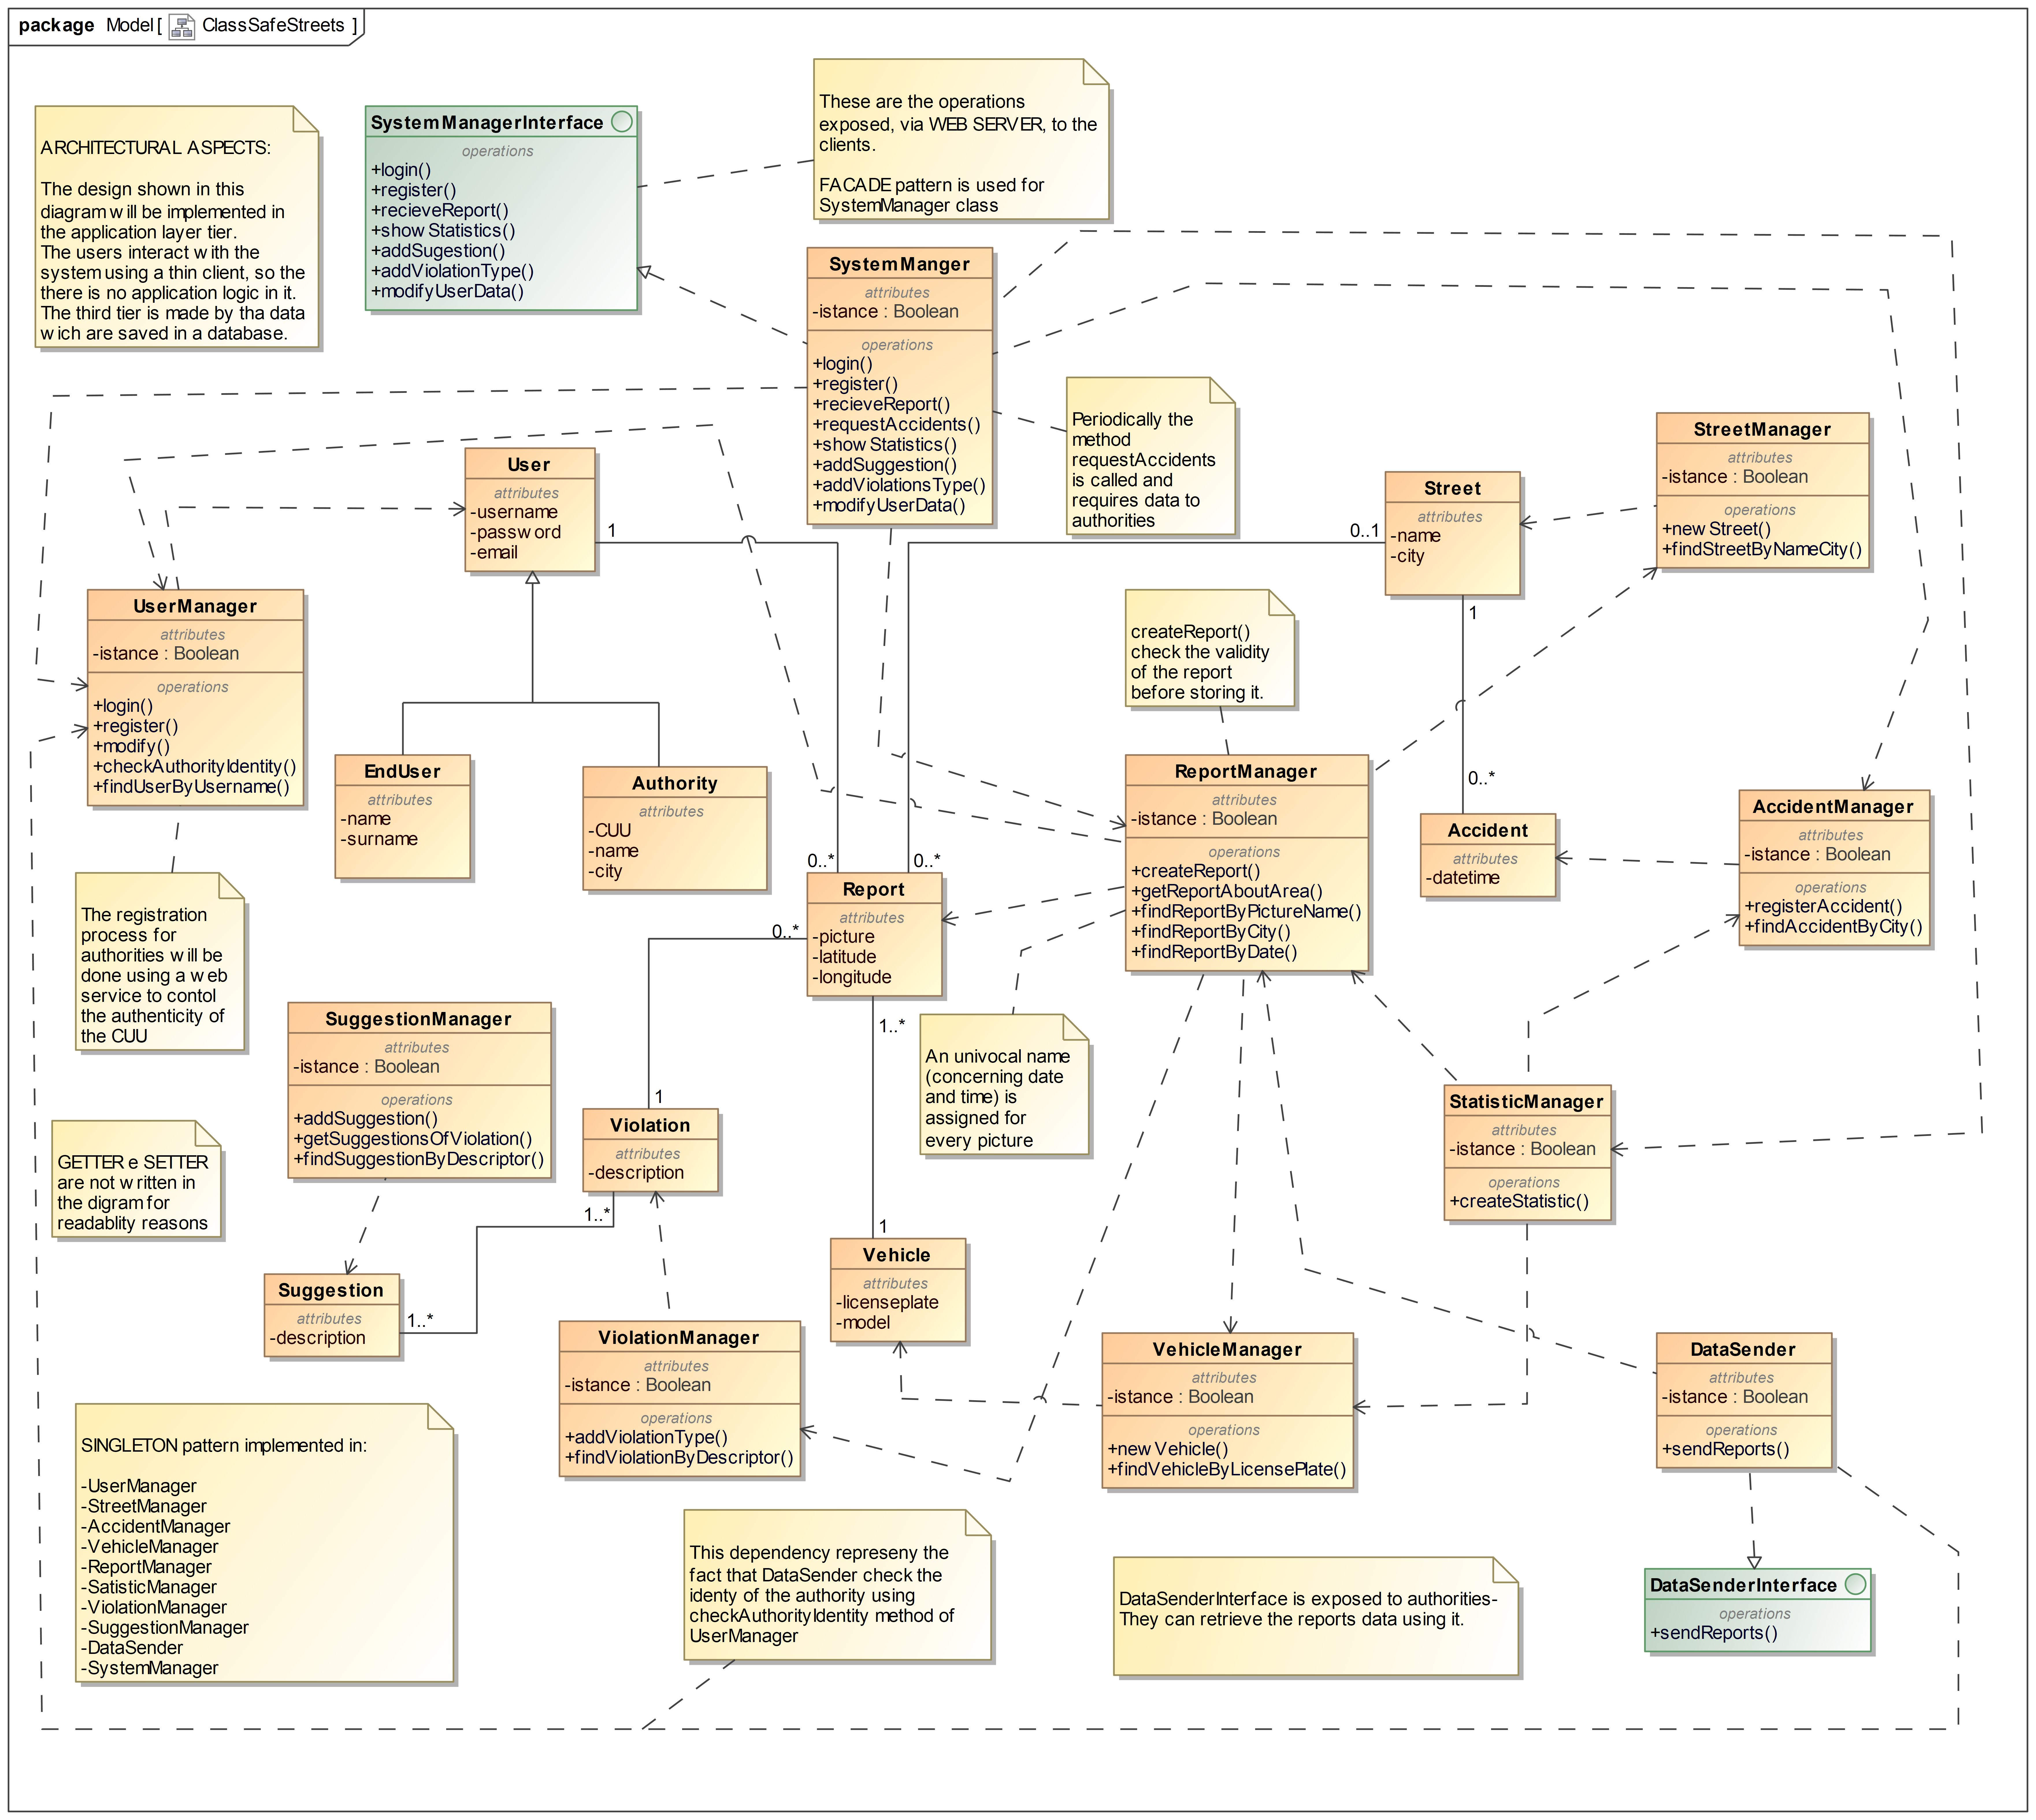
\includegraphics[width=1.12\linewidth]{Images/ClassSafeStreets.png}
	\caption{Class diagram}
\end{figure}

The component diagram below describes the implementation of the classes described before in terms of components.

The macro-component SafeStretsApplication represents the application running on the application server. It exposes two interface. The first one is designed to communicate with the web server that catch the clients requests. The second is exposed to authority systems in order to offer information that can be used to generate traffic tickets.

There are also subcomponents that perform specific operations and interact with the database:
\begin{itemize}
 \item 
 SystemManager: is the component that conveys all the request to the appropriate subcomponents and periodically activate the AccidentManager.
 \item 
 AccidentManager: is the component that calls the specific service to retrieve the data about accidents occured. These informations will be used by StatisticManager.
 \item
 StatisticManager: is the component designed to create statistic crossing data coming from report and accidents.
 \item 
 PositionManager: is the component used to organize data about position and streets.
 \item 
 UserManager: is the component used to manage user operations (for istance login,registration...).
 \item
 ReportSender: it is used to send data about reports stored to authority system. These information will be used to generate traffic tickets. This subcomponent exposes directly an interface to the external enviroment. Naturally before sending the data, the method check the identity of the authority using the UserManager.
 \item 
 VehicleManger: is the component designed to manage the data about vehicle.
 \item 
 ViolationAndSuggestionMangaer: it is used to store and modify the type of violation and suggestion.
 \item 
 ReportMangaer: is the component that store reports in the database and retrive information on it.
 
\end{itemize}

\begin{figure}[H]
	\centering
	\includegraphics[width=1.12\linewidth]{Images/component.png}
	\caption{Component diagram}
\end{figure}

\subsection{Deployment view}
In the deployment diagram below it is possible to see the physical implementation of the system.
SafeStreets is composed by 3 nodes:
\begin{itemize}
	\item 
	First tier: represent the thin clien that make HTTP requests. It is used by users for sending reports and by authorities in order to see statistics.
	\item 
	Second tier: is made by the web server and the appliaction server. The first one is responsible of the catching of the HTTP requests coming from the clients. The web server read the requests and call the appropriate method exposed by the application server. The real computation of the requests is done here.
	When data stored are required, the application server communicates with the third tier.
	\item 
	Second tier: this tier represent the database of the system. 
\end{itemize} 

In the diagram there is also an other node that corresponds with the authority system in charge of retrieving reports to generate traffic tickets. The application server exposes a interface that provides this function. 

\begin{figure}[H]
	\centering
	\includegraphics[width=1.12\linewidth]{Images/Deployment.png}
	\caption{Deployment diagram}
\end{figure}

\subsection{Runtime view}

\subsection{Component interfaces}

The interfaces exposed are manly 2, SystemManagerInterface and DataSenderInterface. Their role was explained in the previuos sections of this document.

\begin{figure}[H]
	\centering
	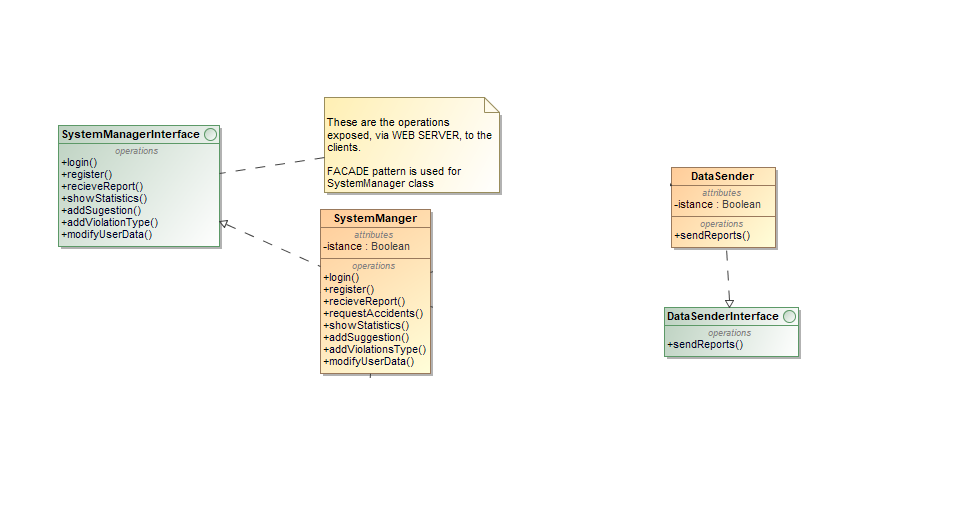
\includegraphics[width=1.12\linewidth]{Images/ComponentInterfaces.png}
	\caption{Component interfaces}
\end{figure}


Here the focus is on the feature provided by the methods exposed.

\subsubsection{SystemManagerInterface}

\begin{itemize}
	\item 
	User login(String user, String password)
	
	is the method in charge of checking of the idenitity of the user/authority that want to log in the application. It returns the object User if the login process was succefully done, if it is not the object is null. The application server checks the type of User object returned and then generate the relative web page (user page or authority page) to return to the client.
	The method works invoking methods of UserManger class.
	
	\item 
	User register(String user, String password, String mail, String name, String surname)
	
	This method does the registration of a normal user and returns the User object as login method. Since the user has to be univocal the process can abort, in this case a null object is returned.
	Reading the returned object, the web server will generate the proper web page.
	The method works invoking methods of UserManger class.
	
	\item 
	User register(String user, String password, String mail, String name, String CUU, String city)
	
	This method does the registration of an authority user and returns the User object as login method. Since the user has to be univocal and the CUU is checked (via Web Service) here, the process can abort, in this case a null object is returned.
	Reading the returned object, the web server will generate the proper web page.
	The method works invoking methods of UserManger class.
	
	\item
	 Bool recieveReport(String picture, Double latitute, Double longitude, String Violation, String violation, String licenseplate, String user, String city, String streetName)
	 
	 This method creates the report. During this process all the checkings concerning the autenticity of the picture are performed and the coordinates are tarsformed into street name and city. In case the operations ends successfully, the proper objects (Report, Vehicle, Street) are created or associated (Violation, User) and then all data will be stored in the database. The picture name will be renamed with an univocal key made on date, time and user. A true value is returned.
	 In case of bad result of the checkings on the authenticity, a false value will be returned.
	 According to the value returned by the method, the web server will generate the proper web page.
	 These operations will be performed using methods of ViolationManager, UserManager, ReportManager, VehicleManager and  StreetManager methods.
	 
	 \item
	List<Integer> showStatistics (String user, String city)
	
	This method before generating statiscs redgarding the city, checks the identity of the user. 
	If the username does not correspond to an authority, it returns a null value.
	Otherwise it generates statistics using data of reports and accidents in the city.
	According to the result of the method the web server generate the proper web page.
	This method works using UserManger and StatisticManager classes.
	
	\item 
	Bool addSuggestion (String user, String description)
	
	This method before adding the suggestion, checks the identity of the user. 
	If the username does not corresponds to an authority, it returns a false value.
	Otherwise it adds the suggestion to the list and returns true.
	According to result of the method the web server generate the proper web page.
	This method wors using UserManger and SuggestionManager classes.
	
	\item 
	Bool addViolationType(String user, String descrption)
	
	This method has the same behaviour of the previus one regarding the suggestions.
	
	\item 
	Bool modifyUserData(String oldPassword, String email, String newpassword)
	
	The method update the data if the username exists and the old password is correct, then
	a boolean value. According to it the web server create the web page.
	The method use UserManager class to perfom that opertaion.
\end{itemize}

\subsubsection{SystemManagerInterface}

The only method of this interface is sendReports:
\hfill

List<Report> sendReport (String username, String password, String city, Date date)



The method checks the identity using the usename and the password. If it results a profile of an authority, a list of report done in the city on that date is provided to the caller. Otherwise a null value is returned.
The process works using ReportManager class and without involving the web server.






